% begin module greatest-integer-function
\begin{frame}
\begin{definition}[Greatest Integer Function]
The \emph{greatest integer function} $\lfloor x\rfloor$ is defined as the largest integer that is less than or equal to $x$.
\end{definition}
In computer science this function is called the \emph{floor} function.
\begin{columns}[c]
\column{.5\textwidth}
\psset{xunit=1cm, yunit=1cm}
\begin{pspicture}(-1.5, -1.5)(3.8,3.8)
\psaxes[labels=x, ticks=x]{<->}(0,0)(-1.5,-1.5)(3.8,3.8)
\psline(-0.1,1)(0.1,1)
\rput[b](-0.25, 1){$1$}
\psline[linecolor=red](-1,-1)(0,-1)
\psFullDot{-1}{-1}
\psHollowDot{0}{-1}

\psline[linecolor=red](0,0)(1,0)
\psFullDot{0}{0}
\psHollowDot{1}{0}

\psline[linecolor=red](1,1)(2,1)
\psFullDot{1}{1}
\psHollowDot{2}{1}

\psline[linecolor=red](2,2)(3,2)
\psFullDot{2}{2}
\psHollowDot{3}{2}

\psline[linecolor=red](3,3)(3.8,3)
\psFullDot{3}{3}
%\psHollowDot{4}{3}
\end{pspicture}
%\ 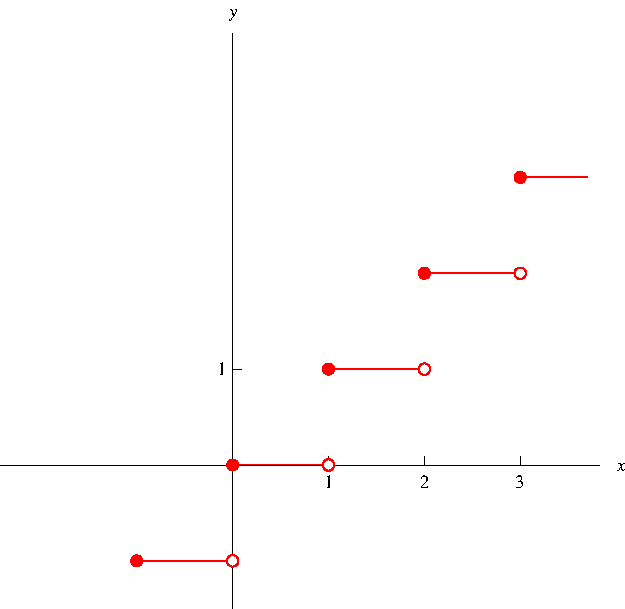
\includegraphics[height=4.5cm]{continuity/pictures/02-05-ex2d.pdf}%

\column{.5\textwidth}
\begin{align*}
\uncover<2->{%
\alert<handout:0| 2-3>{%
\lfloor 
4 
\rfloor
}}%
& \uncover<2->{%
\alert<handout:0| 2-3>{%
 = \uncover<handout:0| 3->{%
 4%
}}}\\%
\uncover<2->{%
\alert<handout:0| 4-5>{%
\lfloor 
4.8%
\rfloor
}}%
& \uncover<2->{%
\alert<handout:0| 4-5>{%
 = \uncover<handout:0| 5->{%
 4%
}}}\\%
\uncover<2->{%
\alert<handout:0| 6-7>{%
\lfloor 
\pi%
\rfloor
}}%
& \uncover<2->{%
\alert<handout:0| 6-7>{%
 = \uncover<handout:0| 7->{%
 3%
}}}\\%
\uncover<2->{%
\alert<handout:0| 8-9>{%
\lfloor 
\sqrt{2}%
\rfloor
}}%
& \uncover<2->{%
\alert<handout:0| 8-9>{%
 = \uncover<handout:0| 9->{%
 1%
}}}\\%
\uncover<2->{%
\alert<handout:0| 10-11>{%
\left\lfloor 
-\frac{1}{2}%
\right\rfloor %
}}%
& \uncover<2->{%
\alert<handout:0| 10-11>{%
 = \uncover<handout:0| 11->{%
-1%
}}}\\%
\uncover<2->{%
\alert<handout:0| 12-13>{%
\left\lfloor 
-\pi%
\right\rfloor %
}}%
& \uncover<2->{%
\alert<handout:0| 12-13>{%
 = \uncover<handout:0| 13->{%
-4%
}}}%
\end{align*}
\end{columns}
\end{frame}
% end module greatest-integer-function
